%  LaTeX support: latex@mdpi.com 
%  In case you need support, please attach all files that are necessary for compiling as well as the log file, and specify the details of your LaTeX setup (which operating system and LaTeX version / tools you are using).

%=================================================================
\documentclass[cryptography,article,submit,moreauthors,pdftex]{Definitions/mdpi}

\firstpage{1} 
\makeatletter 
\setcounter{page}{\@firstpage} 
\makeatother
\pubvolume{xx}
\issuenum{1}
\articlenumber{5}
\pubyear{2020}
\copyrightyear{2020}
%\externaleditor{Academic Editor: name}
\history{Received: date; Accepted: date; Published: date}
%\updates{yes}

%\usepackage[utf8x]{inputenc}
%\usepackage[top=0.5in,left=0.5in,right=0.5in,bottom=0.5in]{geometry}
\usepackage{xcolor}
\usepackage{titlesec}
\usepackage{hyperref}
\usepackage{mathtools}
%\usepackage{amsmath}
\usepackage{amssymb}
\usepackage{amsfonts}
\usepackage{amsthm}
%\usepackage[english]{babel}
\usepackage{caption}
\usepackage{graphicx}
%\graphicspath{{}}
\usepackage{tikz}
\usetikzlibrary{shapes,arrows}

%\theoremstyle{plain}
\newtheorem*{theorem}{Theorem}
\hbadness = 10001

\Title{Enhancing the NTRU cryptosystem}

% Author Orchid ID: enter ID or remove command
\newcommand{\orcidauthorA}{0000-0001-5858-5417} % Add \orcidA{} behind the author's name
\newcommand{\orcidauthorB}{0000-0002-3667-8513} % Add \orcidB{} behind the author's name

% Authors, for the paper (add full first names)
\Author{Awnon Bhowmik $^{1,\dagger,\ddagger}$\orcidA{} and Unnikrishnan Menon $^{1,\ddagger}$\orcidB{}}

% Authors, for metadata in PDF
\AuthorNames{Firstname Lastname, Firstname Lastname and Firstname Lastname}

% Affiliations / Addresses (Add [1] after \address if there is only one affiliation.)
\address{%
$^{1}$ \quad Department of Mathematics and Computer Science, 94-20 Guy R. Brewer Blvd, Jamaica, NY 11451; awnon.bhowmik@yorkmail.cuny.edu\\
$^{2}$ \quad Department of Eletrical and Electronics Engineering, VIT, Vellore Campus, Tiruvalam Rd, Katpadi, Vellore, Tamil Nadu 632014; unnikrishnanr.menon2017@vitstudent.ac.in}

% Contact information of the corresponding author
\corres{Correspondence: awnon.bhowmik@yorkmail.cuny.edu}

% Current address and/or shared authorship
%\firstnote{Current address: Affiliation 3} 
%\secondnote{These authors contributed equally to this work.}
% The commands \thirdnote{} till \eighthnote{} are available for further notes

%\simplesumm{} % Simple summary

%\conference{} % An extended version of a conference paper

% Abstract (Do not insert blank lines, i.e. \\) 
\abstract{NTRU is an open-source public key cryptosystem that uses lattice-based cryptography to
encrypt and decrypt data. Unlike other popular public-key cryptosystems, it is resistant to attacks using Shor's Algorithm and its performance has been shown to be significantly greater. This paper talks about how Koblitz encoding from Elliptic Curve Cryptography (ECC) can be used to convert each character in a dataset to a point on an elliptic curve. A Pythagoras Theorem analogy is used to turn the point to a single number, which is converted to a sequence of coefficients in Z. A polynomial is then generated for each of these characters. Then the polynomial is reduced, and we show that choosing appropriate
parameters for the cryptosystem can make it highly secure and that the decryption algorithm
turns out taking linear time. Since each character is represented by its own polynomial, it
increases obscurity thereby increasing the complexity for decryption and thus the security level. We
also implement a form of data compression and test whether data compression and expansion during the encryption-decryption process results in original data with no or minimal loss.
}

% Keywords
\keyword{post quantum cryptography; lattice based encryption; quantum cryptography; Koblitz encoding; post quantum cryptosystem; ntru cryptography; ntru cryptosystem}


\begin{document}
\section{Why Lattice Cryptography}
\begin{flushleft}
\textbf{The real reason}$^{\text{\cite{security_2017}}}$
\begin{itemize}
    \item In 1994, Shor's Algorithm break RSA and ECC with quantum computers
    \item 2015, NSA announcement: prepare for the quantum apocalypse
    \item 2017, NIST call for competition/standardization
    \item 2030, predicted general purpose quantum computers
\end{itemize}

\textbf{Further usefulness}$^{\text{\cite{security_2017}}}$
\begin{itemize}
    \item Good understanding of underlying hard problem
    \item Fast, parallel-able, hardware friendly
    \item Numerous applications: FHE, ABE, MMap, Obfuscation...
\end{itemize}

\textbf{Data vaulting attack}$^{\text{\cite{security_2017}}}$
\begin{itemize}
    \item A.k.a. harvest-then-decrypt attack
    \item Data needs to be secret for, lets say, 30 years
    \item Quantum computer arrives in, lets say, 15 years
    \item Perhaps the most practical attack in cryptography
\end{itemize}

\newpage
\textbf{Encrypt Schemes}$^{\text{\cite{security_2017}}}$
\begin{itemize}
    \item NTRUEncrypt - standardized by IEEE and ASC X9
\end{itemize}

\textbf{Signature Schemes}$^{\text{\cite{security_2017}}}$
\begin{itemize}
    \item BLISS (NTRU)
    \item pqNTRUSign (NTRU)
\end{itemize}

This paper specifically focuses on the NTRUEncrypt and NTRUDecrypt algorithm.
\end{flushleft}

\section{Koblitz Encoding Algorithm for ECC}
\begin{flushleft}
	The encoding algorithm for ECC is as follows...\\
	\begin{itemize}
		\item Given a message $M$, convert each character $m_k$ into a number $a_k$ using Unicode, where $b=2^{16}$ and $0<a_k<2^{16}$
		\item Convert the message $M$ into an integer using $$m=\sum_{k=1}^n a_kb^{k-1}$$. In practice we choose an $n$ to be less than or equal to $160$ such that $m$ satisfies $m\le 2^{16\cdot 160}<p$.
		\item Fix a number $d$ such that $d\le \dfrac{p}{m}$. In practice we choose the prime $p$ large enough so that we can allow $d=100$.
		\item For integers $j=0,1,2,\cdots d-1$  we do the following loop
		\begin{itemize}
			\item Compute the $x$ coordinate of a point on the elliptic curve as $x_j=(dm+j)\mod p$ where $m=\bigg\lfloor{\dfrac{x_j}{d}}\bigg\rfloor$
			\item Compute $s_j=(x_j^3+Ax+B)\mod p$
			\item If $\left(s_j\right)^{\frac{p+1}{2}}\equiv s_j\mod p$, then define $y$ coordinate of a point on the elliptic curve as $y_j=\left(s_j\right)^{\frac{p+1}{4}}\mod p$. Return the point $(x_j,y_j)$.
		\end{itemize}
	\end{itemize}
	
	Thus we are able to encode our message $M$, as an element of the abelian group $G=E\left(\mathbb{F}_p\right)$ $^{[9]}$
\end{flushleft}

\section{NTRUEncrypt}
NTRU operations are based on objects in a truncated polynomial ring $R=\mathbb{Z}[X]/(X^N-1)$ with convolution multiplication and all polynomials in the ring have integer coefficients and degree at most $N-1$:
\begin{equation}
    \textbf{c}(X)=c_0+c_1X+c_2X^2+\cdots+c_{N-1}X^{N-1}
\end{equation}

\section{Equivalence class modulo 3}
Any number divided by 3 can result in remainders $\left\{0,1,2\right\}$. So any number divided by 3 is one of $3r,3r+1,3r+2$. This is useful in constructing the trinary basis $\left\{-1,0,1\right\}^{\text{dim}}$. The elements in the basis forms the coefficients of the polynomial $(1)$.

\newpage
\begin{theorem}
Let $R\subseteq S\times S$ be an equivalence class on a set $S$. Then the set of $\mathcal{R}$-classes constitutes the whole of $S$
\end{theorem}

\begin{proof}
    \notag
    \begin{align}
        \forall x\in S:x\in[x]_{\mathcal{R}}&\qquad\text{Definition of equivalence class}\\
        \lnot\left(\exists x\in S:x\notin [x]_{\mathcal{R}}\right)&\qquad\text{Assertion of universality}\\
        \lnot\left(\exists x\in S: x\notin\bigcup[x]_{\mathcal{R}}\right)&\qquad\text{Definition of set union}\\
        \forall x\in S:x\in\bigcup S/\mathcal{R}&\qquad\text{Assertion of universality}\\
        S\subseteq\bigcup S/\mathcal{R}&\qquad\text{Definition of subset}
    \end{align}
    
    Also:
    \begin{align}
        \forall X\in S/\mathcal{R}:X\subseteq S&\qquad\text{Definition of equivalence class}\\
        \bigcup S/\mathcal{R}\subseteq S&\qquad\text{Union is smallest superset: general result}
    \end{align}
    By definition of set equality
    $$\bigcup S/\mathcal{R}=S$$
    and so the set of all $\mathcal{R}$-classes constitutes the whole of $S^{\cite{proofwiki}}$.
\end{proof}

\begin{flushleft}
    This theorem tells us that in our case, we are using $\mod 3$ to generate coefficients from the set $\left\{-1,0,1\right\}$ which is basically the numbers of the form $3r-1,3r,3r+1$. It means that the union of all these equivalence classes spans the entire set of integers before modulo reduction.
\end{flushleft}
 
\section{Lattice Cryptography}
\textbf{What is a lattice?}$^{\cite{security_2017}}$
\begin{flushleft}
A \textbf{lattice} consists of all the integral combinations of $d\le n$ linearly independent vectors over $\mathbb{R}$. $$\mathcal{L}=\mathbb{Z}\textbf{b}_1+\cdots+\mathbb{Z}\textbf{b}_d=\left\{\lambda_1\textbf{b}_1+\cdots+\lambda_n\textbf{b}_n:\quad \lambda_i\in\mathbb{Z}\right\}$$ where $d$ is the dimension and $\textbf{B}=\left(\textbf{b}_1,\textbf{b}_2,\cdots,\textbf{b}_n\right)$ is a basis. Here is an example $$\textbf{B}=\left(\begin{array}{ccc}5&\frac{1}{2}&\sqrt{3}\\\frac{3}{5}&\sqrt{2}&1
\end{array}\right)$$

Here $d=2,n=3$ and hence $d\le n$
\end{flushleft}

\begin{itemize}
	\item All crypto talks begin with an image of a dim-2 lattice
	\item There is an infinitude of bases which is formed due to matrix multiplication of \textbf{B} and some other matrix
	\item It involves solving the shortest vector problem (SVP). The exact version of the problem is only known to be NP-hard for randomized reductions.$^{\cite{ajtai1996generating}}$ We have used something similar in our algorithm, but here we calculate the sum of squares rather than the $L^2$ norm.
\end{itemize}

\section{Flow Diagram for Proposed Algorithm}
\begin{center}
    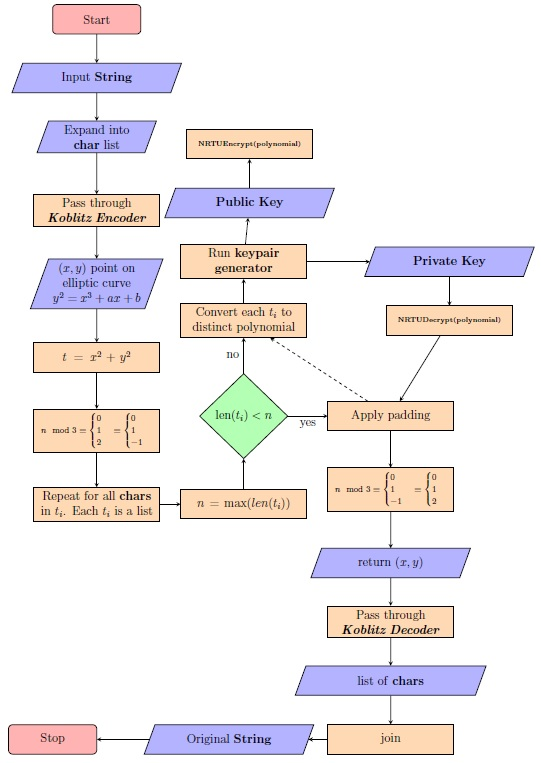
\includegraphics[scale=1.25]{images/Algorithm Flow Diagram.jpg}
\end{center}

\newpage
\section{Proposed Algorithm}
\begin{enumerate}
    \item Input an arbitrary string containing alphanumeric and/or special characters
    \item Split into characters and pass through \textit{Koblitz encoder}
    \item Each character in the string is turned into a point on an elliptic curve $y^2=ax^3+bx+c$, whose parameters $a,b,c$ are user defined
    \item Convert point(s) $(x,y)$ to a single number using the parametrization $t=x^2+y^2$ and apply modulo 3 to turn it into ternary base number. Here $\left\{0,1,2\right\}=\left\{0,1,-1\right\}$. Store these ternary numbers into a list. There should be multiple such lists due to multiple characters in the original string.
    \item Find the maximum size among these lists. For the smaller lists, we apply padding to maintain consistency
    \item Using these ternary values from each list, every character in the string is represented as a polynomial
    \item We generate the public and private keys
    \item Use public key to run NTRUEncrypt() and generate cipher text.
    \item Use private key to run NTRUDecrypt() and obtain original lists of ternary numbers
    \item Reapply padding
    \item Apply a method called ternary\_to\_decimal() to convert the padded lists into $(x,y)$ points
    \item Pass the $(x,y)$ points through \textit{Koblitz Decoder} to obtain the list of characters. Combining these characters, finally allows us to retrieve the original plain text.
\end{enumerate}

\section{An attempt on loss less encoding}
Messages encrypted by the Koblitz method results in a long polynomial. It is safe to assume that the length of this polynomial increases linearly with the length of message. Hence, a modification to the aforementioned algorithm in Fig 1. was attempted by converting the polynomials into a gray scale map to obtain some sort of data compression. Following sample results were obtained.

\begin{center}
		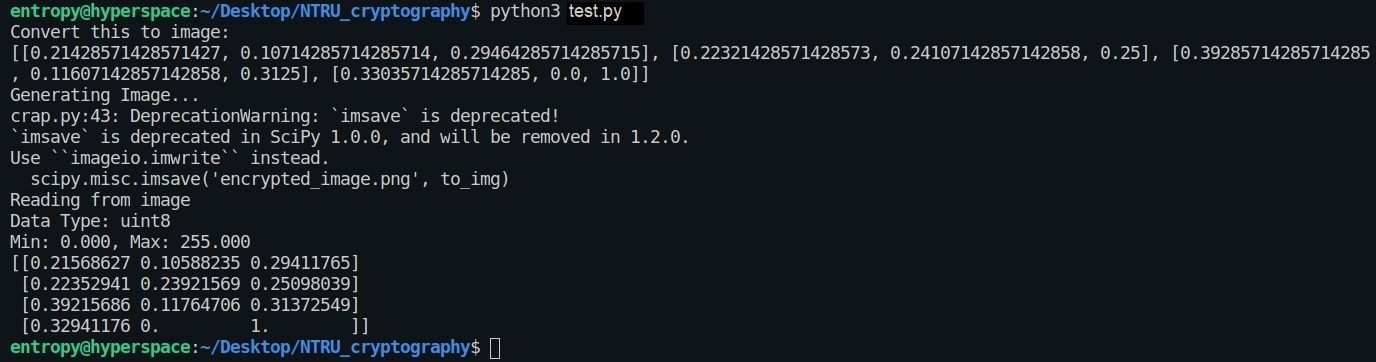
\includegraphics[scale=0.53]{images/Attempt 1.jpg}\captionof*{"Attempt 1".png}{\textbf{Attempt 1}}
		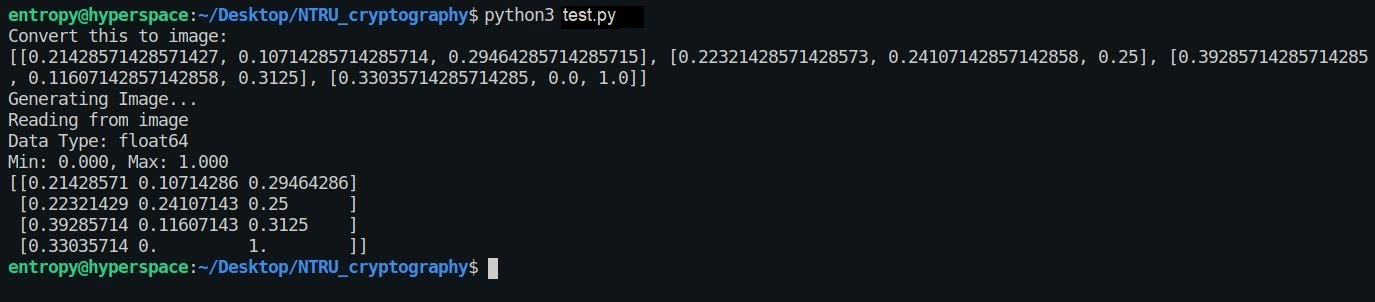
\includegraphics[scale=0.53]{images/Attempt 2.jpg}\captionof*{"Attempt 2".png}{\textbf{Attempt 2}}
\end{center}

\begin{flushleft}
The first attempt involved PNG image format and produced results that were correct up to 2 decimal places only. This means that this format produced a large percentage error. Another thing to notice is that this involved only 8 bit precision unsigned integers. However, using TIFF image format with 64 bit precision unsigned integers resulted in a much better match between the encrypted and the decrypted matrix. Following is a sample gray scale map that was generated.
\end{flushleft}

\begin{center}
	
\includegraphics[scale=0.59]{images/grayscale map.jpg}\captionof*{"grayscale map".jpg}{Fig 2. \textbf{Gray scale map of data compression}}
\end{center}

\begin{flushleft}
\textbf{Remark:} It is to be noted that every character in our input string is treated differently, i.e. if we write the message "banana", then each of the characters have a different random polynomial. The polynomials for all 3 a's and both n's are distinct. This is what makes this cryptosystem more secure.
\end{flushleft}

\section{Finite fields in NTRU}
\begin{flushleft}
Field theory is an essential topic that forms the mathematical foundation of many cryptosystems. The NTRU cryptosystem is no different. The operations involved in our procedure are$^{\text{\cite{latticehacks}}}$

\begin{itemize}
	\item $p,q$ primes, where $p<q$
	\item addition - $f(x)+g(x)$
	\item multiplication - $f(x)\cdot g(x)$
	\item cyclic convolution - $f(x)\cdot g(x) \mod (x^n-1)$
	\item modular reduction - $\left(f(x_i)+\dfrac q2\right)\mod q - \dfrac q2 \quad \forall i\le n$. $n$ is the $\deg(f(x))$
\end{itemize}
\end{flushleft}

\begin{flushleft}
A \textbf{field} $F$, sometimes denoted $\left\{F,+,\times\right\}$ is a set of elements with two binary operation, called \textit{addition} and \textit{multiplication}, such as for all $a,b,c$ in $F$ the following axioms are obeyed.$^{\text{\cite{stallings2017}}}$
\end{flushleft}

\subsection{Properties of finite fields}
\begin{flushleft}
Consider a finite field $\left\{F,+,\times\right\}$. Let $x,y$ be any two arbitrary elements in the field. Then the following properties hold true.
\begin{enumerate}
	\item \textbf{Commutativity}\qquad\quad $\begin{cases}x+y&=y+x\\x\times y&=y\times x\end{cases}$
	\item \textbf{Associativity}\qquad\qquad\, $\begin{cases}x+(y+z)&=(x+y)+z\\x\times(y\times z)&=(x\times y)\times z\end{cases}$
	\item \textbf{Identity}\qquad\qquad\qquad\quad $\begin{cases}0\in F& x+0=0+x=x\\1\in F&1\times x=x\times 1=x\end{cases}$
	\item \textbf{Additive Inverse}\qquad\quad\, For any $x\in F$, there exists $-x\in F$ such that $x+(-x)=0$
	\item \textbf{Distributivity}\qquad\qquad\quad $(x+y)\times z=x\times z+y\times z$
	\item \textbf{Multiplicative Inverse}\quad For any $x\in F,x\neq 0, \exists x^{-1}\in F$ such that $x\times x^{-1}=1$
\end{enumerate}
\end{flushleft}

\begin{flushleft}
It can be shown that the order of a finite field (number of elements in the field) must be a power of a prime $p^n$, where n is a positive integer. The finite field of order $p^n$ is generally written $GF(p^n)$; $GF$ stands for Galois field, in honor of the mathematician who first studied finite fields. Two special cases are of interest for our purposes. For $n = 1$, we have the finite field $GF(p)$; this finite field has a different structure than that for finite fields with $n>1$ and is studied in this section. For finite fields of the form $GF(p^n), GF(2^n)$ fields are of particular cryptographic interest.${^{\text{\cite{stallings2017}}}}$
\end{flushleft}

\section{Result}
\begin{flushleft}
    The following snapshot resembles a sample test run of the entire program.
    \begin{center}
        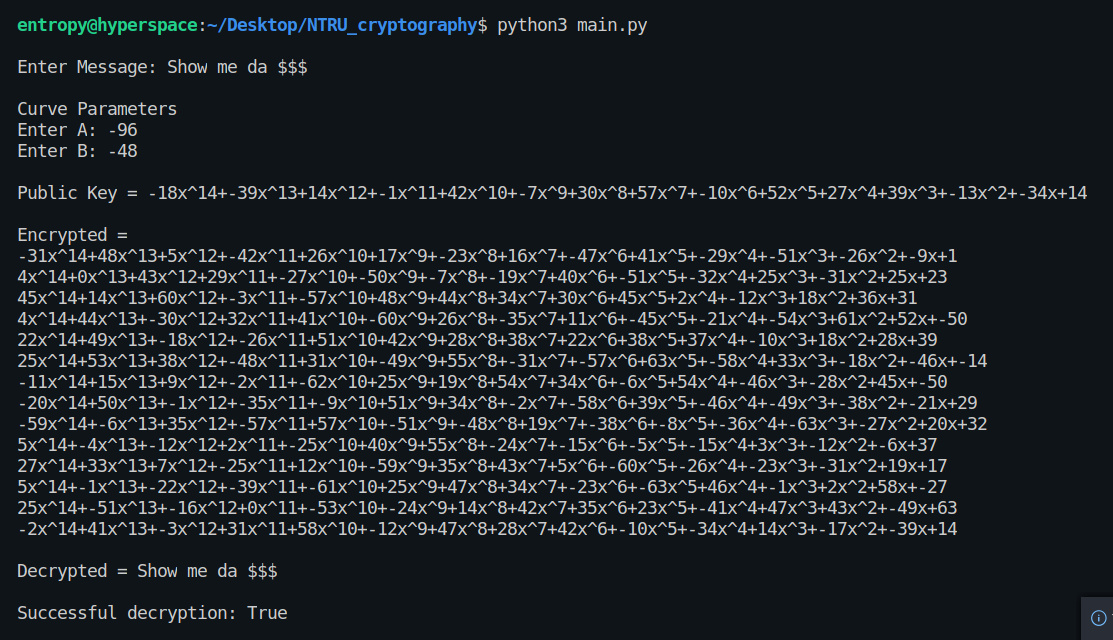
\includegraphics[scale=0.35]{images/Test Run.png}\captionof*{"Test Run".png}{Fig 4. \textbf{Sample test run showing the entire process}}
    \end{center}
\end{flushleft}

\section{Experiments by varying parameters}
\subsection{String length vs time to encrypt/decrypt}
\begin{flushleft}
A function was written on Jupyter Notebook to test out the relationship between string length $s$ (x-axis) and time of encryption/decryption $t_{\text{enc}}/t_{\text{dec}}$ (y-axis).
\begin{center}
	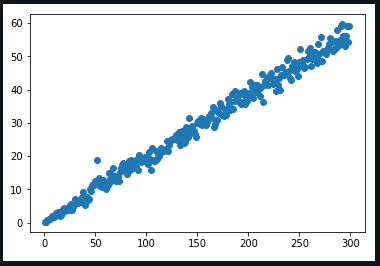
\includegraphics[scale=0.75]{images/strlen vs time.png}\captionof*{"strlen vs time".png}{Fig 3. \textbf{string length vs time to encrypt}}
\end{center}

A best fit shape through these points is a straight line through the \textit{origin}. It can be safely assumed that for an arbitrary string length $s$, time to encrypt $t_{\text{enc}}$ and time to decrypt $t_{\text{dec}}$, we can write
\end{flushleft}

\begin{itemize}
	\centering
	\item $t_{\text{enc}}\propto s$
	\item $t_{\text{dec}}\propto s$
\end{itemize}

\begin{flushleft}
To test the authenticity of our encryption paradigm we fixed elliptic curve parameters $(a,b)=(-96,-48)$. We generated a custom string of length $74$ that contained numeric values, alphabets (upper and lower case), special characters, spaces etc and generated $100$ new strings by randomly shuffling the elements of this custom string. It was observed that for each of the $100$ test cases, we were able to successfully retrieve the original message after completing an encrypt-decrypt cycle
\end{flushleft}

\subsection{Valid elliptic parameters vs String length}
\begin{enumerate}
	\item We take a custom string of length $74$. This consists of all alphnumeric characters, special characters and space.
	\item We run a $O(n^2)$ complexity loop to check for $(a,b)$ in range $[-100,100]$.
	\item Due to lack of recommended processing power, we break out of the loop as soon as the first combination is found. The combination turned out to be $(a,b)=(-96,-48)$
	\item We shuffled the original string $100$ times to make $100$ different strings of length $74$.
	\item For each of the shuffled strings, we only consider the first 20 characters due to shortage of processing power. So basically we now have $100$ strings of length $20$ that comprises of any random character on the English keyboard.
	\item We run the encrypt-decrypt function on these strings. The job of the encrypt-decrypt function is to return true only if the decrypted message matches perfectly with the input plaintext.
\end{enumerate}

\begin{flushleft}
We observed that for each of the $100$ test cases, the encrypt-decrypt function returns true.
\end{flushleft}

\section{Conjecture}
\begin{enumerate}
	\item The elliptic curve parameter $(a,b)=(-96,-48)$ works irrespective of the string length of the message and the type of characters present in the string.
	\item $(a,b)=(-96,-48)$ is one of the many combinations of elliptic curve parameter that works. Proof of this is dependent on greater computational power.
\end{enumerate}

\section{Future Work}
\begin{flushleft}
We are planning to wrap up the entire program into a pip install package which would be available for general public use. NTRU algorithm has been around for a while but there is still no official implementation of this algorithm in libraries such as pycryptodome. We would love to see our version of NTRU becoming a part of this library. It will serve as a great security layer against post quantum cryptography. We would also like to incorporate this crypto system as a security layer for a web socket based client server chat app, built with Tkinter. For the moment, the work we have done so far has been compiled into a repository$^{\cite{ntru}}$. We have also noticed that using the numpy module makes quick work of calculations which we have coded from scratch. This would also fix some formatting issues to make the encrypted polynomial more legible.
\end{flushleft}

\reftitle{References}
\begin{thebibliography}{999}
% Reference 1
\bibitem[Author1(year)]{security_2017}
A Short Review of the NTRU Cryptosystem. {\em O. Security} {\textbf{July 2017}}, \\Available online: \href{https://www.slideshare.net/OnBoardSecurity/a-short-review-of-the-ntru-cryptosystem}{https://www.slideshare.net/OnBoardSecurity/a-short-review-of-the-ntru-cryptosystem}
% Reference 2
\bibitem[Author2(year)]{proofwiki}
Union of Equivalence Classes is Whole Set.\\Available online: \href{https://proofwiki.org/wiki/Union_of_Equivalence_Classes_is_Whole_Set}{https://proofwiki.org/wiki/Union\_of\_Equivalence\_Classes\_is\_Whole\_Set}
% Reference 3
\bibitem[Author2(year)]{latticehacks}
NTRU. Available online: \href{https://latticehacks.cr.yp.to/ntru.html}{https://latticehacks.cr.yp.to/ntru.html}
% Reference 4
\bibitem[Author2(year)]{stallings2017}Stallings, W.; \em{The principles and Practice of Cryptography and Network Security 7th Edition, ISBN-10: 0134444280} \em{Pearson Education} \textbf{2017}
% Reference 5
\bibitem[Author3(year)]{ajtai1996generating} Ajtai, M.; \em{Generating hard instances of lattice problems}, \em{Proceedings of the twenty-eighth annual ACM symposium on Theory of computing}; pp 99-108
% Reference 6
\bibitem[Author4(year)]{ntru} Bhowmik, A. \& Menon, U.; \textit{NTRU Cryptography}, {\textbf{2020}}. \\Available online: \href{https://github.com/7enTropy7/NTRU_cryptography}{https://github.com/7enTropy7/NTRU\_cryptography}
\end{thebibliography}
\end{document}